%% This Beamer template is based on the one found here: https://github.com/sanhacheong/stanford-beamer-presentation, and edited to be used for Stanford ARM Lab

\documentclass[10pt, aspectratio=169]{beamer}
%\mode<presentation>{}

\usepackage{media9}
\usepackage{amssymb,amsmath,amsthm,enumerate}
\usepackage[utf8]{inputenc}
\usepackage{array}
\usepackage[parfill]{parskip}
\usepackage{graphicx}
\usepackage{caption}
\usepackage{subcaption}
\usepackage{bm}
\usepackage{amsfonts,amscd}
\usepackage[]{units}
\usepackage{listings}
\usepackage{multicol}
\usepackage{multirow}
\usepackage{tcolorbox}
\usepackage{physics}

% Enable colored hyperlinks
\hypersetup{
    colorlinks=true,
    citecolor=uma_pink,
    linkcolor=uma_blue_light,
    filecolor=uma_blue_water,      
    urlcolor=uma_blue_light,
    pdftitle={Overleaf Example},
    pdfpagemode=FullScreen,
}

\renewcommand{\thebibliography}{\textcolor{uma_blue_water}{\arabic{bibliography}}}
\renewcommand{\thefigure}{\textcolor{uma_blue_water}{\arabic{figure}}}
\renewcommand{\figurename}{\textcolor{uma_blue_water}{Fig.}}
\renewcommand{\thesubfigure}{\textcolor{uma_blue_water}{\alph{subfigure}}}
\renewcommand{\thetable}{\textcolor{uma_blue_water}{\arabic{table}}}
\renewcommand{\tablename}{\textcolor{uma_blue_water}{Table}}


% The following three lines are for crossmarks & checkmarks
\usepackage{pifont}% http://ctan.org/pkg/pifont
\newcommand{\cmark}{\ding{51}}%
\newcommand{\xmark}{\ding{55}}%

% Numbered captions of tables, pictures, etc.
\setbeamertemplate{caption}[numbered]

%\usepackage[superscript,biblabel]{cite}
\usepackage{algorithm2e}
\renewcommand{\thealgocf}{}

% Bibliography settings
\usepackage[style=ieee]{biblatex}
\setbeamertemplate{bibliography item}{\insertbiblabel}
\addbibresource{references.bib}

% Glossary entries
\usepackage[acronym]{glossaries}
\newacronym{ML}{ML}{machine learning}
\newacronym{HRI}{HRI}{human-robot interactions}
\newacronym{RNN}{RNN}{Recurrent Neural Network}
\newacronym{LSTM}{LSTM}{Long Short-Term Memory}


\theoremstyle{remark}
\newtheorem*{remark}{Remark}
\theoremstyle{definition}

\newcommand{\empy}[1]{{\color{uma_blue_dark}\emph{#1}}}
\newcommand{\empr}[1]{{\color{uma_blue_dark}\emph{#1}}}
\newcommand{\examplebox}[2]{
\begin{tcolorbox}[colframe=uma_blue_dark,colback=uma_gray_light,title=#1]
#2
\end{tcolorbox}}

\usetheme{Uma} 
\def \i  {\item}
\def \ai {\item[] \quad \arrowbullet}
\newcommand \si[1]{\item[] \quad \bulletcolor{#1}}
\def \wi {\item[] \quad $\ \phantom{\Rightarrow}\ $}
\def \bi {\begin{itemize}\item}
\def \ei {\end{itemize}}
\def \be {\begin{equation*}}
\def \ee {\end{equation*}}
\def \bie {$\displaystyle{}
\def \eie {{\ }$}}
\def \bsie {\small$\displaystyle{}
\def \esie {{\ }$}\normalsize\selectfont}
\def \bse {\small\begin{equation*}}
\def \ese {\end{equation*}\normalsize}
\def \bfe {\footnotesize\begin{equation*}}
\def \efe {\end{equation*}\normalsize}
\renewcommand \le[1] {\\ \medskip \lefteqn{\hspace{1cm}#1} \medskip}
\def \bex {\begin{example}}
\def \eex {\end{example}}
\def \bfig {\begin{figure}}
\def \efig {\end{figure}}
\def \btheo {\begin{theorem}}
\def \etheo {\end{theorem}}
\def \bc {\begin{columns}}
\def \ec {\end{columns}}
\def \btab {\begin{tabbing}}
\def \etab {\end{tabbing}\svneg\svneg}
\newcommand \col[1]{\column{#1\linewidth}}
\def\vneg  {\vspace{-5mm}}
\def\lvneg {\vspace{-10mm}}
\def\svneg {\vspace{-2mm}}
\def\tvneg {\vspace{-1mm}}
\def\vpos  {\vspace{5mm}}
\def\lvpos {\vspace{10mm}}
\def\svpos {\vspace{2mm}}
\def\tvpos {\vspace{1mm}}
\def\hneg  {\hspace{-5mm}}
\def\lhneg {\hspace{-10mm}}
\def\shneg {\hspace{-2mm}}
\def\thneg {\hspace{-1mm}}
\def\hpos  {\hspace{5mm}}
\def\lhpos {\hspace{10mm}}
\def\shpos {\hspace{2mm}}

\logo{
\includegraphics[height=0.8cm]{./style_files_uma/logo_uma_negativo}\hspace{0.1cm}}

% commands to relax beamer and subfig conflicts
% see here: https://tex.stackexchange.com/questions/426088/texlive-pretest-2018-beamer-and-subfig-collide
\makeatletter
\let\@@magyar@captionfix\relax
\makeatother

\title[\href{https://jmgandarias.com}{\textcolor{white}{jmgandarias.com}}]{Cartesian Trajectory Planning}

%\subtitle{Subtitle Of Presentation}

%\beamertemplatenavigationsymbolsempty

\begin{document}

\author[Systems Engineering and Automation]{
	\large
	Juan M. Gandarias\\
    \footnotesize \href{mailto:jmgandarias@uma.es}{jmgandarias@uma.es}
}

\institute{
	\textcolor{uma_gray_dark}{
    Systems Engineering and Automation Department\\
	University of Malaga\\
    \href{https://www.uma.es/imech/}{IMECH.UMA}}
 	\vskip 5pt
    % \small{\date{\today}}
 %    \begin{figure}
	% 	\centering
	% 	\begin{subfigure}[t]{0.5\textwidth}
	% 		\centering
	% 		
\includegraphics[height=1.5cm]{./style_files_uma/logo_uma}
	% 	\end{subfigure}%
	% 	~
	% 	\begin{subfigure}[t]{0.5\textwidth}
	% 		\centering
	% 		\includegraphics[height=0.33in]{./images/arm_lab_logo_with_title_small_adj_6.png}
	% 	\end{subfigure}
	% \end{figure}
}


\date{\today}

\begin{noheadline}
\begin{frame}
    \maketitle
    \vspace{-1cm}
    \begin{figure}
		\centering
		
\includegraphics[height=1.5cm]{./style_files_uma/logo_uma}
        \hspace{10cm}
        
\includegraphics[height=1.4cm]{./style_files_uma/logo_isa}
	\end{figure}
 %    \begin{figure}
	% 	\centering
	% 	\begin{subfigure}[t]{0.5\textwidth}
	% 		\centering
	% 		
\includegraphics[height=1.5cm]{./style_files_uma/logo_uma}
	% 	\end{subfigure}%
	% 	~
	% 	\begin{subfigure}[t]{0.5\textwidth}
	% 		\centering
	% 		\includegraphics[height=0.33in]{./images/arm_lab_logo_with_title_small_adj_6.png}
	% 	\end{subfigure}
	% \end{figure}
 \end{frame}
\end{noheadline}



\setbeamertemplate{itemize items}[default]
\setbeamertemplate{itemize subitem}[circle]

\begin{frame}
	\frametitle{Overview} % Table of contents slide, comment this block out to remove it
	\tableofcontents % Throughout your presentation, if you choose to use \section{} and \subsection{} commands, these will automatically be printed on this slide as an overview of your presentation
\end{frame}

\section{Introduction}
% `[allowframebreaks]` can be used to have multiple slides in one frame, where the slides are continued with the suffix "(cont.)"; `[allowframebreaks]` can be used with `\framebreak` to manually break each frame into multiple slides
\begin{frame}[allowframebreaks]
\frametitle{Introduction}
	Itemize example
	\begin{itemize}
		\item Item 1
		\item Item 2
        \begin{table}[]
        \caption{Example of Table - Taxonomy of human intent prediction}
        \label{tab:table_example}
        \vspace{-.75cm}
        \resizebox{0.95\textwidth}{!}{%
        \begin{tabular}{|c|c|c|c|}
        \hline
        \multicolumn{2}{|c|}{\multirow{2}{*}{Human}} & \multicolumn{2}{c|}{\begin{tabular}[c]{@{}c@{}}Execution Strategy\\ (Action)\end{tabular}}                            \\ \cline{3-4} 
        \multicolumn{2}{|c|}{}                       & \begin{tabular}[c]{@{}c@{}}Observer\\ Knows\end{tabular} & \begin{tabular}[c]{@{}c@{}}Observer\\ Unknown\end{tabular} \\ \hline
        \multirow{2}{*}{\begin{tabular}[c]{@{}c@{}}Objective \\ Function\end{tabular}} &
          \begin{tabular}[c]{@{}c@{}}Observer\\ Knows\end{tabular} &
          \begin{tabular}[c]{@{}c@{}}All is Known (e.g. Ping Pong) \\ where both objective and actions are clear\end{tabular} &
          \begin{tabular}[c]{@{}c@{}}Human Action Model is unclear\\  or suboptimal (e.g. chess)\end{tabular} \\ \cline{2-4} 
         &
          \begin{tabular}[c]{@{}c@{}}Observer\\ Unknown\end{tabular} &
          \begin{tabular}[c]{@{}c@{}}Human action model is well known, \\ but objective is not (e.g. joy-riding in car \\ or free running, where destination\\  or direction is unclear)\end{tabular} &
          \begin{tabular}[c]{@{}c@{}}Poor action model and objective\\  function (e.g. Poor / good cook, \\ no idea of final dish)\end{tabular} \\ \hline
        \end{tabular}%
        }
        \end{table}

		\item Tables can be referenced as Table  \ref{tab:table_example}
	\end{itemize}
	
	\framebreak
	
	Example of a figure, shown in Figure \ref{fig:prob_formulation_scenario_1}.
	
	\begin{figure}
        \centering
        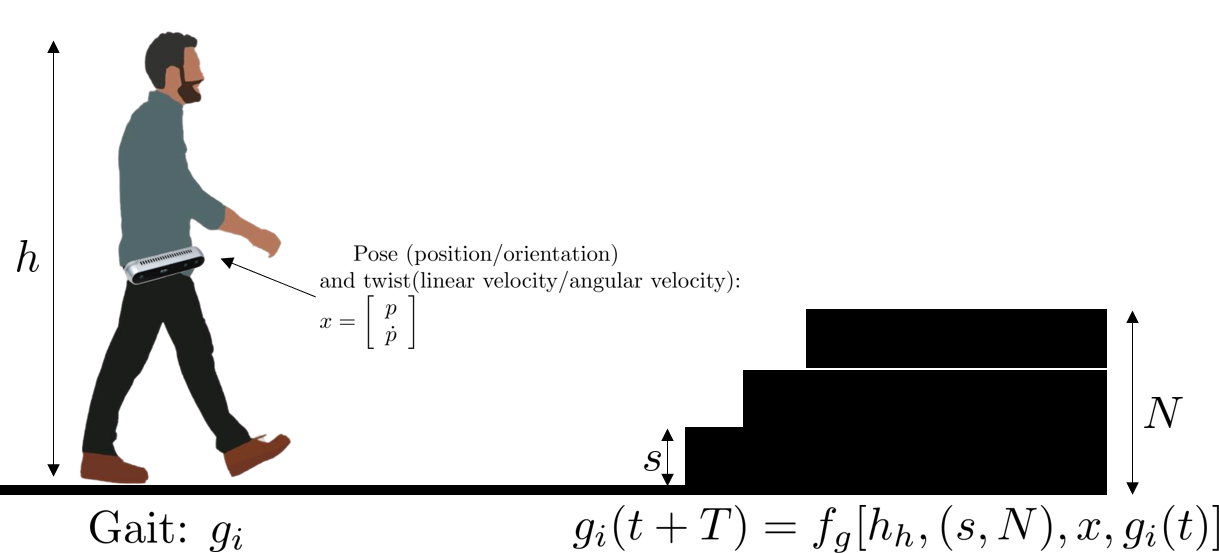
\includegraphics[width=0.8\textwidth]{images/prob_formulation_scenario_1.png}
        \caption{Example Figure}
        \label{fig:prob_formulation_scenario_1}
    \end{figure}
\end{frame}

% This demonstrates a new section
\section{Examples}
% This demonstrates a single frame without framebreaks
\begin{frame}{Example of Horizontal Subfigures}

	\begin{figure}
		\centering
		\begin{subfigure}[t]{0.5\textwidth}
			\centering
			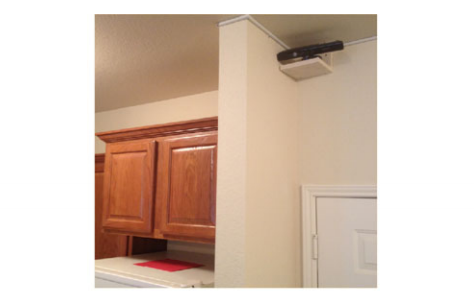
\includegraphics[width=0.9\textwidth]{images/stone2014fall_setup.png}
			\caption{Single Kinect setup for fall prevention in elderly residence \cite{stone2014fall}}
		\end{subfigure}%
		~ 
		\begin{subfigure}[t]{0.5\textwidth}
			\centering
			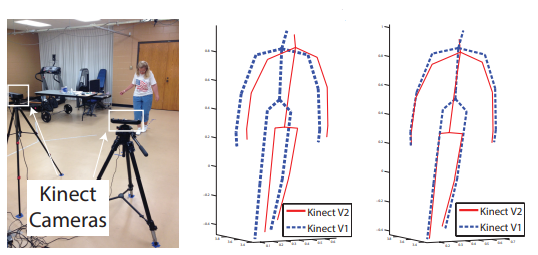
\includegraphics[width=\textwidth]{images/staranowicz2015easy_multiple_kinects.png}
			\caption{Multiple Kinects calibration for fall prediction\cite{staranowicz2015easy}}
		\end{subfigure}
		\caption{Examples of Horizontal Subfigures}
	\end{figure}
\end{frame}

\begin{frame}{Example of Horizontal Alignment}
    % For data collection:
    
    Example of Horizontal Alignment of a \texttt{table} and a \texttt{figure}.
    \begin{center}
    \begin{minipage}[t]{.65\linewidth}
    \begin{table}[H]
    % \renewcommand{\arraystretch}{1.3}
    \caption{Environment limitations on data collection}
    \label{tab:env_limit}
    \centering
    % \begin{tabular}{m{1.6cm}|c|>{\centering\arraybackslash}m{2cm}|>{\centering\arraybackslash}m{2.3cm}}
    \begin{tabular}{m{2cm}|c|c|>{\centering\arraybackslash}m{1.5cm}}
    % \begin{tabular}{c|c|c|c}
        & Kinect & Stereo & Kinect + Stereo\\
        \hline
        Indoor & \cmark & \cmark & \cmark \\
        \hline
        Outdoor & \xmark & \cmark & \cmark \\
        \hline
        High number of features & \cmark & \cmark & \cmark \\
        \hline
        Low number of features & \cmark & \xmark & \cmark 
    \end{tabular}
    \end{table}
    \end{minipage}%
    \begin{minipage}[t]{.35\linewidth}
    \vspace{0pt}
    \centering
    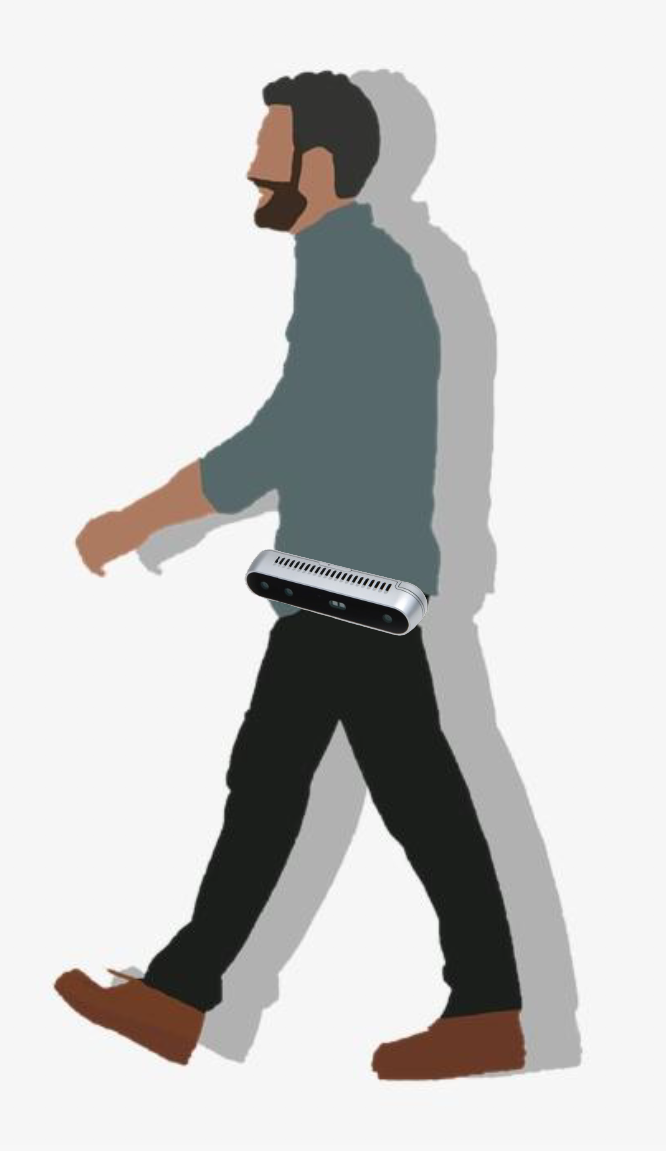
\includegraphics[width=0.7\textwidth]{images/waist_cam_setup_new.png}
    \end{minipage}
    \end{center}
\end{frame}

\begin{frame}[allowframebreaks]
\frametitle{Example of resizable equations}

\begin{center}
\scalebox{1.0}{\parbox{\linewidth}{%
		\begin{align*}
		& {\text{min \hskip 6pt}}
		& & J = \int (a_{real} - \hat{a})^2  \\
		& \text{subject to}
		& & \text{human kinematics} \\
		&&& \text{no collision} \\
		&&& \text{no falling} 
		\end{align*}
}}
\end{center}
\end{frame}

\begin{frame}[allowframebreaks]
\frametitle{Example of Regular Equations}
    % \begin{equation}
    %     {}^Ag = {}^AR_B {}^Bg
    % \end{equation}
    
    % \begin{equation}
    %     V = \frac{{}^Bg \cross {}^Ag}{\norm{{}^Ag}\norm{{}^Bg}}, 
    %     \theta = \arccos{\frac{{}^Bg \cross {}^Ag}{\norm{{}^Ag}\norm{{}^Bg}}}
    % \end{equation}
    
    \begin{equation}
        \begin{split}
        {}^AR_{B}(t_0)=\left[\begin{array}{ccc}
        1 & 0 & 0 \\
        0 & 1 & 0 \\
        0 & 0 & 0
        \end{array}\right]+
        \sin (\theta)\left[\begin{array}{ccc}
        0 & -v_{3} & v_{2} \\
        v_{3} & 0 & -y_{1} \\
        -v_{2} & v_{1} & 0
        \end{array}\right]+ \\
        (1-\cos (\theta))\left[\begin{array}{ccc}
        0 & -v_{3} & v_{2} \\
        v_{3} & 0 & -v_{1} \\
        -v_{2} & v_{1} & 0
        \end{array}\right]^{2}
        \end{split}
        \end{equation}
        
        \begin{align}
            {}^AR_{B}(t) &= \Delta R {}^AR_{B}(t_0) \\
            \Delta R &= {}^AR_{B}(t) {}^AR_{B}^T(t_0)
        \end{align}
\end{frame}

\begin{frame}[allowframebreaks]
\frametitle{Example of Video}

	\includemedia[
	width=\linewidth,
	totalheight=0.6\linewidth,
	activate=pageopen,
	passcontext,  %show VPlayer's right-click menu
	addresource=videos/opensim_video.mp4,
	flashvars={
		%important: same path as in `addresource'
		source=videos/opensim_video.mp4
	}
	]{}{VPlayer.swf}
    
\end{frame}

\begin{frame}[allowframebreaks]
\frametitle{Bibliography}
\printbibliography
\end{frame}

\end{document}